\documentclass[../../main.tex]{subfiles}
\graphicspath{{../../image/}{../../figure/}}
\begin{document}

\section{变分自编码器}\label{section:ch19-变分自编码器}

在本章中，我们将从确定性的自编码器开始学习，然后推广到学习编码器分布 $p(z\mid x)$ 以及解码器分布 $p(y\mid z)$ 的随机模型。这些概率模型称为\textbf{变分自编码器}（variational autoencoder），它们代表了我们训练非线性潜变量模型的 $4$ 种方法中的第 $3$ 种（参见 16.4.4 小节）。

考虑一个生成式模型，其条件分布 $p(x\mid z,w)$ 覆盖了由深度神经网络输出控制的 $D$ 维数据变量 $x$。例如，$g(z,w)$ 可能表示高斯条件分布的均值。同时考虑 $M$ 维潜变量 $z$ 的分布，它由零均值、单位方差的高斯分布给出：
\begin{align}
p(z)=\mathcal{N}(z\mid 0,I)
\label{align:ch19-pz}
\end{align}
潜变量模型的似然函数由下式给出：
\begin{align}
p(x\mid w)=\int p(x\mid z,w)\,p(z)\,\mathrm{d}z
\label{align:ch19-marginal}
\end{align}
其中 $p(x\mid z,w)$ 由一个深度神经网络定义。这个似然函数是难以处理的，因为关于 $z$ 的积分无法解析计算。变分自编码器（Variational AutoEncoder, VAE）（Kingma and Welling, 2013; Rezende, Mohamed, and Wierstra, 2014; Doersch, 2016; Kingma and Welling, 2019）在训练模型时使用了这个似然函数的近似表示来解决这一难题。VAE 背后的关键思想如下：(1) 使用证据下界来近似似然函数，从而与 EM 算法形成紧密联系；(2) 借助摊销推断（即使用编码器网络）来近似 E 步骤中潜变量上的后验分布，而不是精确评估每个数据点的后验分布；(3) 使用重参数化（reparameterization trick）技巧实现编码器模型的可微分训练（参见 15.3 节）。

为了推导出 VAE 的近似，首先回想一下，对于由潜变量 $z$ 描述的空间上的任意概率分布 $q(z)$，以下关系成立（参见 15.4 节）：
\begin{align}
\ln p(x\mid w)=\mathcal{L}(w)+\mathrm{KL}\big(q(z)\,\|\,p(z\mid x,w)\big)
\label{align:ch19-elbo-decomp}
\end{align}
其中 $\mathcal{L}$ 是\textbf{证据下界}（evidence lower bound）或 ELBO，也称变分下界（variational lower bound），由下式给出：
\begin{align}
\mathcal{L}(w)=\int q(z)\ln\Big\{\frac{p(x\mid z,w)\,p(z)}{q(z)}\Big\}\,\mathrm{d}z
\label{align:ch19-elbo}
\end{align}
Kullback--Leibler 散度（简称 KL 散度）$\mathrm{KL}(q\|p)$ 定义如下：
\begin{align}
\mathrm{KL}\big(q(z)\,\|\,p(z)\big)=-\int q(z)\ln\Big\{\frac{p(z)}{q(z)}\Big\}\,\mathrm{d}z
\label{align:ch19-kl}
\end{align}
由于 KL 散度满足 $\mathrm{KL}(q\|p)\ge 0$，可以得到
\begin{align}
\ln p(x\mid w)\ge \mathcal{L}
\label{align:ch19-elbo-lower}
\end{align}
所以 $\mathcal{L}$ 是 $\ln p(x\mid w)$ 的证据下界。虽然对数似然函数 $\ln p(x\mid w)$ 难以直接计算，但我们可以使用蒙特卡洛估计方法来评估这个下界，从而使它近似于真实对数似然函数的值。

考虑从模型分布 $p(x)$ 中独立采样的训练数据集 $\mathcal{D}=\{x_1,\cdots,x_N\}$。这个数据集的对数似然函数由下式给出：
\begin{align}
\ln p(\mathcal{D}\mid w)=\sum_{n=1}^{N}\mathbb{E}_{q(z_n\mid x_n,\phi)}\Big[\ln p(x_n\mid z_n,w)\Big]-\sum_{n=1}^{N}\mathrm{KL}\big(q(z_n\mid x_n,\phi)\,\|\,p(z_n)\big)
\label{align:ch19-total-elbo}
\end{align}

\subsection{摊销推理}\label{subsection:ch19-摊销推理}

请注意，这引入了与每个数据向量 $x_n$ 相对应的单独潜变量 $z_n$，就像我们在混合模型和概率 PCA 模型中看到的那样。因此，每个潜变量都有自己的独立分布 $q_n(z_n)$，且都可以单独优化（参见 15.2 节和 16.2 节）。

对于深度生成式模型，精确后验分布由贝叶斯定理给出：
\begin{align}
p(z\mid x,w)=\frac{p(x\mid z,w)\,p(z)}{\int p(x\mid z,w)\,p(z)\,\mathrm{d}z}
\label{align:ch19-posterior}
\end{align}
其中分子是可以直接计算的。然而分母是由似然函数给出的，难以解析计算。因此，我们需要找到一个对后验分布的近似。原则上，我们可以为每个分布 $q_n(z_n)$ 单独建立参数化模型，并进行数值优化，但计算成本非常高，特别是对于大数据集来说，此外还需要在每次更新 $w$ 后重新计算分布。因此，我们决定换一个方向，引入第二个神经网络来探索一个更有效的近似框架。

在变分自编码器中，我们不再单独为每个数据点 $x_n$ 计算一个后验分布 $p(z\mid x_n,w)$，而是通过训练一个称为\textbf{编码器网络}的神经网络来近似所有这些分布。这种技术称为\textbf{摊销推理}（amortized inference），要求编码器生成单一的分布 $q(z\mid x,\phi)$，该分布以 $x$ 为条件，其中 $\phi$ 代表网络参数。由证据下界给出的目标函数现在同时依赖于 $\phi$ 和 $w$，我们可以使用基于梯度的优化方法来联合优化这两组参数。

因此，VAE 包含两个参数独立但能联合训练的神经网络：一个编码器网络，用于将数据向量映射到潜空间；一个解码器网络，用于将潜空间向量映射回数据空间。类似于简单的神经网络自编码器模型，所不同的是，我们在潜空间中定义了一个概率分布。我们将看到，编码器根据贝叶斯定理计算解码器的近似概率逆过程——即根据给定观测数据推断潜变量的分布。

在变分自编码器中，编码器的一个典型选择是具有对角协方差矩阵的高斯分布，其均值 $\mu_n$ 和方差 $\sigma_n^2$ 由一个以 $x$ 作为输入的神经网络给出：
\begin{align}
q(z\mid x_n,\phi)=\mathcal{N}\big(z\mid \mu(x_n,\phi),\,\sigma^2(x_n,\phi)\,I\big)
\label{align:ch19-encoder}
\end{align}
请注意，均值 $\mu(x,\phi)$ 位于区间 $(-\infty,\infty)$，因此相应的输出单元激活函数可以是线性的；而方差 $\sigma^2(x,\phi)$ 必须是非负的，所以相关的输出单元通常使用指数函数 $\exp(\cdot)$ 作为激活函数。

我们的优化目标是使用基于梯度的优化方法，针对参数 $\phi$ 和 $w$ 最大化这个下界，这通常使用基于小批量数据的随机梯度下降法来实现。尽管是联合优化参数，但从概念上我们可以交替地优化 $\phi$ 和 $w$，如图~\ref{fig:ch19-elbo-opt} 所示。

\begin{figure}[htbp]
\centering
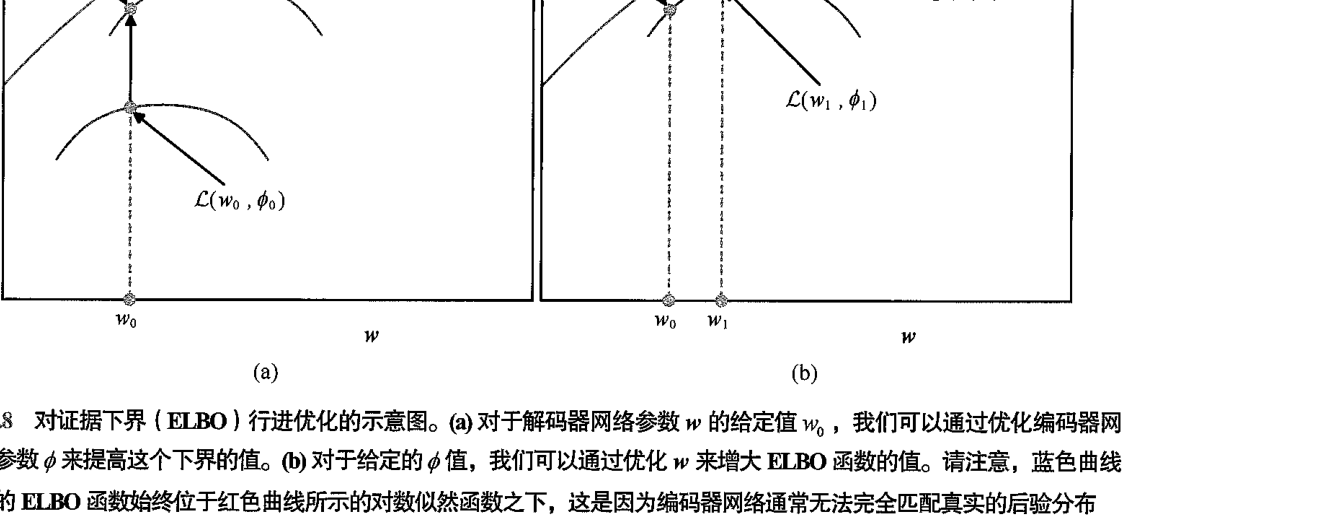
\includegraphics[width=0.85\textwidth]{ch19-fig517-elbo-opt.png}
\caption{对证据下界（ELBO）进行优化的示意图。(a) 对于解码器网络参数 $w$ 的给定值，我们可以通过优化编码器网络的参数 $\phi$ 来提高这个下界的值。(b) 对于给定的 $\phi$ 值，我们可以通过优化 $w$ 来增大 ELBO 函数的值。蓝色曲线所示的 ELBO 函数始终位于红色曲线所示的对数似然函数之下，这是因为编码器网络通常无法完全匹配真实的后验分布。}
\label{fig:ch19-elbo-opt}
\end{figure}

ELBO 优化与 EM 算法的一个关键区别是，对于给定的 $w$ 值，相对于编码器参数 $\phi$ 的优化通常不会将 KL 散度降低到零，因为编码器网络并不能完美地预测后验潜在分布，所以下界和真实对数似然之间存在残差。尽管基于深度神经网络的编码器非常灵活，但它并不能精确地模拟真实的后验分布，原因如下：(1) 真实的条件后验分布未必服从因子分解的高斯分布；(2) 即使是一个大型神经网络，也存在灵活性方面的限制；(3) 训练过程只是一个近似的优化。

\subsection{重参数化技巧}\label{subsection:ch19-重参数化}

遗憾的是，到目前为止，下界 [式~\eqref{align:ch19-elbo}] 仍然难以直接计算，因为在潜变量 $z$ 的积分过程中，解码器网络会导致被积函数对潜变量存在复杂的依赖关系。对于数据点 $x_n$，其对下界的贡献可以表示为：
\begin{align}
\mathcal{L}(w,\phi)=\int q(z\mid x_n,\phi)\ln p(x_n\mid z,w)\,\mathrm{d}z-\mathrm{KL}\big(q(z\mid x_n,\phi)\,\|\,p(z)\big)
\label{align:ch19-point-elbo}
\end{align}

对于式~\eqref{align:ch19-point-elbo}，我们可以尝试用一个简单的蒙特卡洛估计法来近似潜变量 $z$ 上的积分：
\begin{align}
\int q(z\mid x_n,\phi)\ln p(x_n\mid z,w)\,\mathrm{d}z\approx \frac{1}{L}\sum_{l=1}^{L}\ln p(x_n\mid z^{(l)},w)
\label{align:ch19-monte-carlo}
\end{align}
其中 $z^{(l)}$ 是从编码器分布 $q(z\mid x_n,\phi)$ 中采样。关于 $w$ 求导很容易，但关于 $\phi$ 求梯度却存在问题，因为参数 $\phi$ 的变化也会改变采样分布 $q(z\mid x_n,\phi)$。然而这些样本是固定值，所以我们没有办法获取这些样本相对于 $\phi$ 的导数。从概念上讲，我们可以认为将潜变量 $z$ 固定到特定样本值的过程阻止了误差信号向编码器网络的反向传播，如图~\ref{fig:ch19-reparam-block} 所示。

\begin{figure}[htbp]
\centering
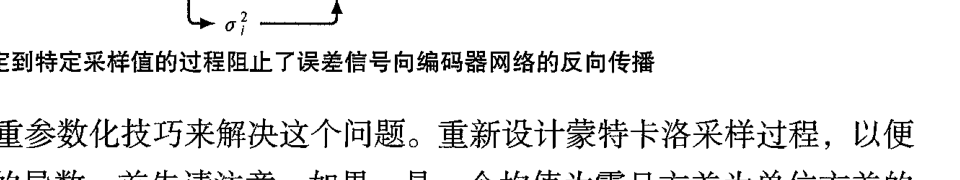
\includegraphics[width=0.8\textwidth]{ch19-fig519-reparam-block.png}
\caption{将潜变量 $z$ 固定到特定采样值的过程阻止了误差信号向编码器网络的反向传播。}
\label{fig:ch19-reparam-block}
\end{figure}

我们可以使用\textbf{重参数化技巧}来解决这个问题。重新设计蒙特卡洛采样过程，以便明确计算相对于 $\phi$ 的导数。首先请注意，如果 $\epsilon$ 是一个均值为零且方差为单位方差的高斯随机变量，那么 $z$ 将具有均值为 $\mu$、方差为 $\sigma^2$ 的高斯分布（见习题 19.2）：
\begin{align}
z=\mu+\sigma\odot\epsilon
\label{align:ch19-reparam}
\end{align}
将其应用于式~\eqref{align:ch19-encoder} 的采样过程，其中 $\mu$ 和 $\sigma$ 由编码器网络的输出 $\mu(x_n,\phi)$ 和 $\sigma^2(x_n,\phi)$ 确定。我们不直接从潜变量 $z$ 采样，而是对 $\epsilon$ 采样，并使用式~\eqref{align:ch19-reparam} 计算对应的 $z$ 样本：
\begin{align}
z^{(l)}=\mu(x_n,\phi)+\sigma(x_n,\phi)\odot\epsilon^{(l)},\qquad \epsilon^{(l)}\sim\mathcal{N}(0,I)
\label{align:ch19-reparam-sample}
\end{align}
其中 $l=1,\cdots,L$ 是样本的索引。该方法显式建立 $\phi$ 与采样值之间的依赖关系，使梯度计算可行，如图~\ref{fig:ch19-reparam-flow} 所示。

\begin{figure}[htbp]
\centering
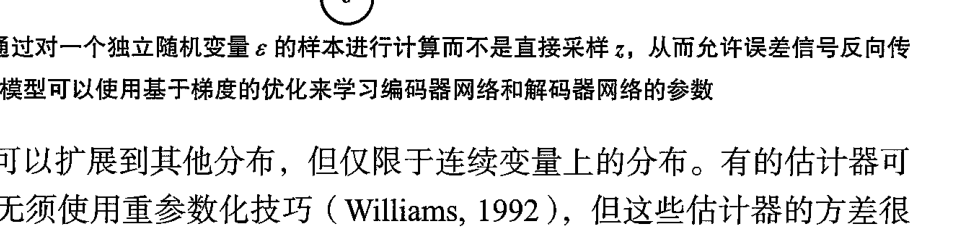
\includegraphics[width=0.8\textwidth]{ch19-fig519-reparam-flow.png}
\caption{重参数化技巧通过对一个独立随机变量 $\epsilon$ 的样本进行计算，而不是直接采样 $z$，从而允许误差信号反向传播到编码器网络。得到的模型可以使用基于梯度的优化来学习编码器网络和解码器网络的参数。}
\label{fig:ch19-reparam-flow}
\end{figure}

使用我们特定的建模假设，VAE 的完整损失函数变为
\begin{align}
\mathcal{L}(w,\phi)\approx\frac{1}{L}\sum_{l=1}^{L}\ln p(x_n\mid z^{(l)},w)-\frac{1}{2}\sum_{j=1}^{M}\big(1+\ln\sigma_j^2(x_n,\phi)-\mu_j^2(x_n,\phi)-\sigma_j^2(x_n,\phi)\big)
\label{align:ch19-full-loss}
\end{align}
其中 $z^{(l)}=\sigma(x_n,\phi)\odot\epsilon^{(l)}+\mu(x_n,\phi)$。每个数据点 $x_n$ 的样本数 $L$ 通常设置为 $1$，即仅使用单个样本进行估计。尽管这种设置会导致对证据下界的计算结果存在噪声，但由于随机梯度优化过程本身就具有噪声，该策略在整体上仍能实现更高效的参数优化。

我们可以将 VAE 训练总结如下。对于小批量中的每个数据点，通过编码器网络前向传播来计算近似潜变量分布的均值和方差，并使用重参数化技巧从该分布中采样，然后将这些样本通过解码器网络传播以计算证据下界 [式~\eqref{align:ch19-full-loss}]。最后使用自动微分计算相对于 $w$ 和 $\phi$ 的梯度。一旦模型训练完成，编码器网络就被丢弃，新的数据点将通过从先验分布 $p(z)$ 中采样并通过解码器网络前向传播来生成数据空间中的样本。

VAE 有许多变种。当应用于图像数据时，编码器通常基于卷积操作，而解码器则基于转置卷积（有时也称反卷积）操作（参见 10.5.3 小节）。在条件 VAE 中，编码器和解码器都将一个条件变量 $c$ 作为额外的输入。例如，我们可能想要生成物体的图像，此时 $c$ 代表物体的类别。潜空间的先验分布 $p(z)$ 既可以是一个简单的高斯分布，也可以扩展成另一个神经网络给出的条件分布 $p(z\mid c)$，训练与测试过程与之前类似。

注意，式~\eqref{align:ch19-point-elbo} 中的第一项鼓励编码器分布 $q(z\mid x,\phi)$ 接近先验分布 $p(z)$，从而使解码器在生成模式下，通过从 $p(z)$ 采样，能够产生逼真的输出。在训练 VAE 时，可能会出现一个问题，即变分分布 $q(z\mid x,\phi)$ 收敛到先验分布 $p(z)$，这意味着变分分布没有从输入 $x$ 中学到有价值的信息。实际上，潜在编码被忽略了，因为它对输入 $x$ 没有区分能力。这称为\textbf{后验崩塌}（posterior collapse）。此时，如果我们取一个输入并编码，然后解码，我们将得到一个看起来模糊不清的重建结果。在这种情况下，KL 散度 $\mathrm{KL}(q(z\mid x,\phi)\|p(z))$ 接近于零。

另一种问题发生在潜在编码没有被压缩的情况下，具体表现是，即使能得到高度准确的重建结果，但从 $p(z)$ 采样并通过解码器网络生成的输出质量却很差，不像训练数据。在这种情况下，KL 散度相对较大，并且因为训练系统获得了一个与先验分布完全不同的变分分布，从先验分布中采样的样本不会生成逼真的输出。这两个问题都可以通过在式~\eqref{align:ch19-point-elbo} 的第一项前引入一个系数 $\beta$ 来解决，以控制 KL 散度的正则化效果，通常 $\beta>1$（Higgins et al., 2017）。如果重建结果很差，则可以增大 $\beta$；而如果生成的样本很差，则可以减小 $\beta$。$\beta$ 的值也可以根据退火调度来设置，即它从一个小的值开始，并在训练期间逐渐增大。

最后请注意，虽然我们在本章中只讨论了一个表示高斯输出分布均值的解码器网络 $g(z,w)$，但我们可以扩展 VAE，让它包含代表高斯分布方差的输出，或进一步让它表示其他更复杂分布的参数，以描绘更广泛多变的数据特征（参见 6.5 节）。

\end{document}